% ===============================================
%                 Chapter 1A.1
%  Techniques for Measuring the Rate of Reaction
%             Created by Michael Tang
%                  2024.12.30
% ===============================================

\subsubsection{1A Techniques for Measuring the Rate of Reaction}
\paragraph{What is an Element?}
\begin{itemize}
    \item \textbf{Definition of an Element:} A pure substance that cannot be broken down into simpler substances through
    chemical reactions.
    \begin{itemize}
        \item It consists of only one type of atom.
        \item Represented on the \underline{Periodic Table} (元素周期表) by a one or two-letter symbol. Example: \ce{H} for
        hydrogen, \ce{Ne} for neon.
    \end{itemize}
    \item \textbf{Periodic Table}
    \begin{figure}[H]
        \centering
        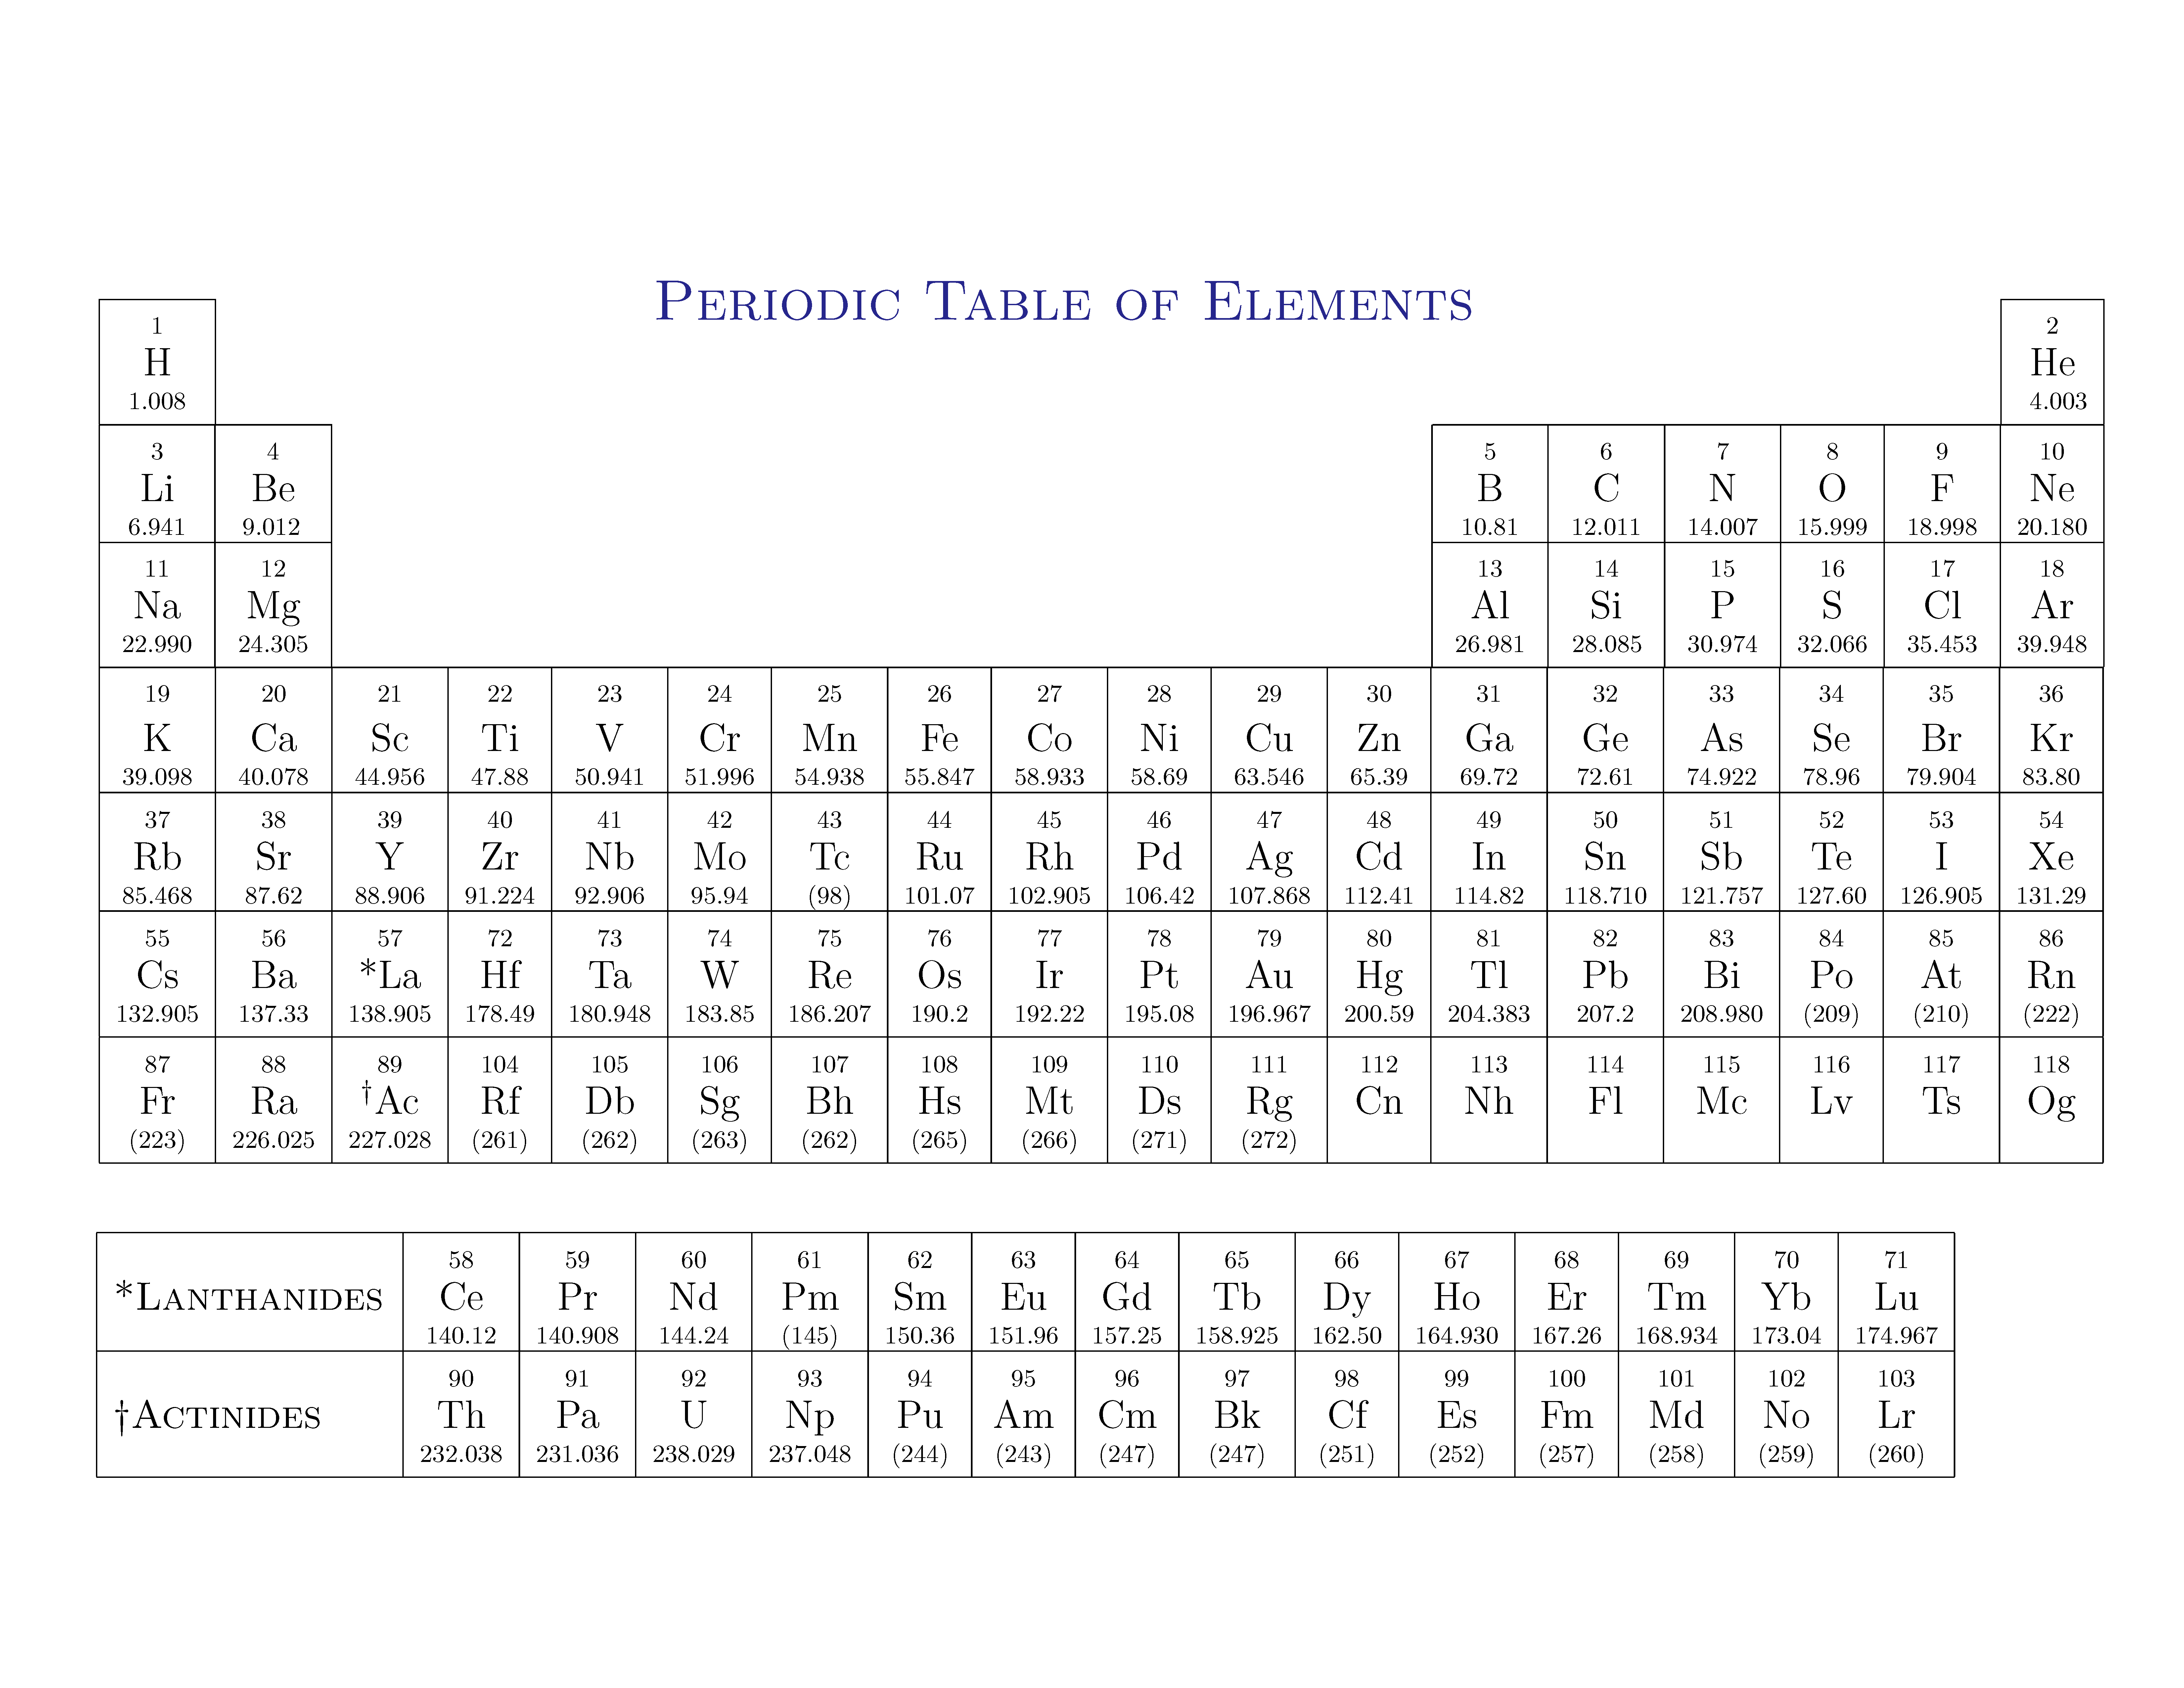
\includegraphics[scale=0.05]{Chemistry/Images/periodic_table.png}
        \caption{Full set of Periodic Table}
    \end{figure}
    \begin{itemize}
        \item[1.]       [Nonmetals]             Hydrogen        氢  (\ce{H})
        \item[2.]       [Nonmetals]             Helium          氦  (\ce{He})
        \item[3.]       [Metals]                Lithum          锂  (\ce{Li})
        \item[4.]       [Metals]                Beryllium       钡  (\ce{Be})
        \item[5.]       [Metalloids]            Boron           硼  (\ce{B})
        \item[6.]       [Nonmetals]             Carbon          碳  (\ce{C})
        \item[7.]       [Nonmetals]             Nitrogen        氮  (\ce{N})
        \item[8.]       [Nonmetals]             Oxygen          氧  (\ce{O}) 
        \item[9.]       [Nonmetals]             Fluorine        氟  (\ce{F})
        \item[10.]      [Nonmetals]             Neon            氖  (\ce{Ne})
        \item[11.]      [Metals]                Sodium          钠  (\ce{Na})
        \item[12.]      [Metals]                Magnesium       镁  (\ce{Mg})
        \item[13.]      [Metals]                Aluminium       铝  (\ce{Al})
        \item[14.]      [Metalloids]            Silicon         硅  (\ce{Si})
        \item[15.]      [Nonmetals]             Phosphorus      磷  (\ce{P})
        \item[16.]      [Nonmetals]             Sulfur          硫  (\ce{S}) 
        \item[17.]      [Nonmetals]             Chlorine        氯  (\ce{Cl})
        \item[18.]      [Nonmetals]             Argon           氩  (\ce{Ar})
        \item[19.]      [Metals]                Potassium       钾  (\ce{K})
        \item[20.]      [Metals]                Calcium         钙  (\ce{Ca})
        \item[21.]      [Transition Metals]     Scandium        钪  (\ce{Sc})
        \item[22.]      [Transition Metals]     Titanium        钛  (\ce{Ti})
        \item[23.]      [Transition Metals]     Vanadium        钒  (\ce{V})
        \item[24.]      [Transition Metals]     Chromium        铬  (\ce{Cr})
        \item[25.]      [Transition Metals]     Manganese       锰  (\ce{Mn})
        \item[26.]      [Transition Metals]     Iron            铁  (\ce{Fe})
        \item[27.]      [Transition Metals]     Cobalt          钴  (\ce{Co})
        \item[28.]      [Transition Metals]     Nickel          镍  (\ce{Ni})
        \item[29.]      [Transition Metals]     Copper          铜  (\ce{Cu})
        \item[30.]      [Transition Metals]     Zinc            锌  (\ce{Zn})
        \item[31.]      [Metals]                Gallium         镓  (\ce{Ga})
        \item[32.]      [Metalloids]            Germanium       锗  (\ce{Ge})
        \item[33.]      [Metalloids]            Arsenic         砷  (\ce{As})
        \item[34.]      [Nonmetals]             Selenium        硒  (\ce{Se})
        \item[35.]      [Nonmetals]             Bromine         溴  (\ce{Br})
        \item[36.]      [Nonmetals]             Krypton         氪  (\ce{Kr})
        \item[37.]      [Metals]                Rubidium        铷  (\ce{Rb})
        \item[38.]      [Metals]                Strontium       锶  (\ce{Sr})
        \item[39.]      [Transition Metals]     Yttrium         钇  (\ce{Y})
        \item[40.]      [Transition Metals]     Zirconium       锆  (\ce{Zr})
        \item[41.]      [Transition Metals]     Niobium         铌  (\ce{Nb})
        \item[42.]      [Transition Metals]     Molybdenum      钼  (\ce{Mo})
        \item[43.]      [Transition Metals]     Technetium      锝  (\ce{Tc})
        \item[44.]      [Transition Metals]     Ruthenium       钌  (\ce{Ru})
        \item[45.]      [Transition Metals]     Rhodium         铑  (\ce{Rh})
        \item[46.]      [Transition Metals]     Palladium       钯  (\ce{Pd})
        \item[47.]      [Transition Metals]     Silver          银  (\ce{Ag})
        \item[48.]      [Transition Metals]     Cadmium         镉  (\ce{Cd})
        \item[49.]      [Metals]                Indium          铟  (\ce{In})
        \item[50.]      [Metals]                Tin             锡  (\ce{Sn})
        \item[51.]      [Metalloids]            Antimony        锑  (\ce{Sb})
        \item[52.]      [Metalloids]            Tellurium       碲  (\ce{Te})
        \item[53.]      [Nonmetals]             Iodine          碘  (\ce{I})
        \item[54.]      [Nonmetals]             Xenon           氙  (\ce{Xe})
        \item[55.]      [Metals]                Caesium         铯  (\ce{Cs})
        \item[56.]      [Metals]                Barium          钡  (\ce{Ba})
        \item[57-71]    [Not In Consideration]
        \item[72.]      [Transition Metals]     Hafnium         铪  (\ce{Hf})
        \item[73.]      [Transition Metals]     Tantalum        钽  (\ce{Ta})
        \item[74.]      [Transition Metals]     Tungsten        钨  (\ce{W})
        \item[75.]      [Transition Metals]     Rhenium         铼  (\ce{Re})
        \item[76.]      [Transition Metals]     Osmium          锇  (\ce{Os})
        \item[77.]      [Transition Metals]     Iridium         铱  (\ce{Ir})
        \item[78.]      [Transition Metals]     Platinum        铂  (\ce{Pt})
        \item[79.]      [Transition Metals]     Gold            金  (\ce{Au})
        \item[80.]      [Transition Metals]     Mercury         汞  (\ce{Hg})
        \item[81.]      [Transition Metals]     Thallium        铊  (\ce{Tl})
        \item[82.]      [Metals]                Lead            铅  (\ce{Pb})
        \item[83.]      [Metals]                Bismuth         铋  (\ce{Bi})
        \item[84.]      [Metals]                Polonium        钋  (\ce{Po})
        \item[85.]      [Nonmetals]             Astatine        砹  (\ce{At})
        \item[86.]      [Nonmetals]             Radon           氡  (\ce{Rn})
        \item[87.]      [Metals]                Francium        锄  (\ce{Fr})
        \item[88.]      [Metals]                Radium          镭  (\ce{Ra})
        \item[88-103]   [Not In Consideration]
        \item[104.]     [Transition Metals]     Rutherfordium   鲥  (\ce{Rf})
        \item[105.]     [Transition Metals]     Dubnium         镝  (\ce{Db})
        \item[106.]     [Transition Metals]     Seaborgium      坦  (\ce{Sg})
        \item[107.]     [Transition Metals]     Bohrium         波  (\ce{Bh})
        \item[108.]     [Transition Metals]     Hassium         哈  (\ce{Hs})
        \item[109-118]  [Not In Consideration] 
    \end{itemize}
    \item \textbf{Perodic Table Representation}
    \begin{itemize}
        \item Each box in the Periodic Table corresponds to an element. The symbol for an element is followed by the following
        rules:
        \begin{itemize}
            \item[1.] \textbf{First letter:} Always capitalized.
            \item[2.] \textbf{Second letter (if any):} Always lowercase.
        \end{itemize}
        \item The Periodic Table organizes elements based on their atomic number and properties. The table is divided into
        \underline{groups} (族) and \underline{periods} (周期). Every element in a group has similar properties, and every
        element in a period has the same number of outermost electron shells.
    \end{itemize}
    \item \textbf{Examples from Everyday Life}
    \begin{itemize}
        \item \textbf{Oxygen (\ce{O2} 氧气):} Essential for \underline{respiration} (呼吸) and \underline{combustion} (燃烧).
        \item \textbf{Iron (\ce{Fe} 铁):} Used in construction and manufacturing.
    \end{itemize}
    \item \textbf{Chemical Simplicity:} Elements are chemically the simplest substances.
    \begin{itemize}
        \item Example: Neon (\ce{Ne} 氖) contains only neon atoms and cannot be further simplified chemically.
        \item Water (\ce{H2O} 水) is not an element, as it can be broken down into hydrogen (\ce{H} 氢) and oxygen (\ce{O} 氧).
    \end{itemize}
    \item \textbf{\underline{Isotopes} (同位素) of Elements:} Some elements have isotopes, which are atoms of the same element
    with the same number of \underline{protons} (质子) but a different number of \underline{neutrons} (中子). For example, neon
    contains three stable isotopes, \ce{_{10}^{20}Ne}, \ce{_{10}^{21}Ne}, and \ce{_{10}^{22}Ne}. Note that the number of protons
    and is always the same for isotopes of the same element, but the number of neutrons can \underline{vary} (不同). The number
    of neutrons is usually write as a \underline{superscript} (写在化学符号上脚的) to the left of the element symbol, and the number
    of protons is written as a \underline{subscript} (写在化学符号下脚的) to the left of the element symbol.
\end{itemize}

\paragraph{What is an Atom?}
\begin{itemize}
    \item An atom is the smallest particle of an element that \underline{retains} (保持) the properties of that element.
    \item Atoms are extremely small and cannot be seen with the \underline{naked eye} (肉眼). For example, a \underline{grain}
    (粒) of sand contains about 10,000,000,000,000,000,000 (billions of) atoms of silicon (\ce{Si}) and oxygen (\ce{O}).
    \item An atom is made up of \underline{subatomic particles} (亚原子粒子), including \underline{protons} (质子),
    \underline{neutrons} (中子), and \underline{electrons} (电子). The protons and neutrons are located in the \underline{nucleus}
    (原子核) of the atom, while the electrons orbit the nucleus in \underline{shells} (壳层).
    \item Aroms are fundamental units in chemistry and play a crucial role in understanding elements and their behavior.
\end{itemize}

\paragraph{What is a Molecule?}
\begin{itemize}
    \item A molecule is a group of two or more atoms \underline{chemically bonded} (化学键合) together.
    \item Molecules an be of:
    \begin{itemize}
        \item \textbf{\underline{Elements} (单质):} Molecules consisting of the same type of atom. Example: \ce{O2} (oxygen gas)
        or \ce{H2} (hydrogen gas).
        \begin{figure}[H]
            \centering
            \chemfig{O=O} \hspace{1cm} \chemfig{H-H}
            \caption{Molecule formula of oxygen gas (on the left) and hydrogen gas (on the right).}
        \end{figure}
        \item \textbf{\underline{Compounds} (化合物):} Molecules made of different types of atoms bonded together. Example:
        \ce{H2O} (water) or \ce{CO2} (carbon dioxide).
        \begin{figure}[H]
            \centering
            \chemfig{H-[:30]O-[:-30]H} \hspace{1cm} \chemfig{C=[:30]O=[:-30]O}
            \caption{Molecule formula of water (on the left) and carbon dioxide (on the right).}
        \end{figure}
    \end{itemize}
    \item The formula of a molecule gives the number and type of atoms it contains, e.g., \ce{H2O} contains 2 hydrogen atoms and
    1 oxygen atom.
\end{itemize}

\paragraph{What is a Compound?}
\begin{itemize}
    \item A compound is a substance formed when atoms of two or more diferent elements chemically combine in fixed
    \underline{proportions} (比例).
    \item Compounds have unique properties \underline{distinct} (独特) from the individual elements that from them.
    \item Example:
    \begin{itemize}
        \item \textbf{Water (\ce{H2O}):} Contains hydrogen and oxygen atoms.
        \begin{figure}[H]
            \centering
            \chemfig{H-[:30]O-[:-30]H}
            \caption{Molecule formula of water.}
        \end{figure}
        \item \textbf{Sodium chloride (\ce{NaCl}):} Contains sodium and chlorine atoms.
        \begin{figure}[H]
            \centering
            \chemfig{Na-Cl}
            \caption{Molecule formula of sodium chloride.}
        \end{figure}
    \end{itemize}
    \item Compounds may consist of large numbers of bonded atoms, forming molecules or giant structures.
    \item Types:
    \begin{itemize}
        \item \textbf{Molecular compounds:} Consist of distinct molecules (e.g., water \ce{H2O}, methane \ce{CH4}).
        \item \textbf{Ionic compounds:} Consist of ions (charged particles) arranged in \underline{lattices} (晶格) structures
        (e.g., sodium chloride \ce{NaCl}, magnesium oxide \ce{MgO}).
        \begin{figure}[H]
            \centering
            \chemfig{C(-[2]H)(-[4]H)(-[6]H)(-[0]H)}
            \caption{Molecule formula of methane.}
        \end{figure}
    \end{itemize}
\end{itemize}

\paragraph{What is and Ion?}
\begin{itemize}
    \item An ion is a species consisting of one or more atoms that have gained or lost electrons, resulting is a positive or
    negative charge.
    \item Types of Ions:
    \begin{itemize}
        \item \textbf{\underline{Cations} (阳离子):} An ion with a positive charge, formed by losing electrons (e.g., \ce{Na+},
        \ce{Ca^2+}).
        \item \textbf{\underline{Anions} (阴离子):} An ion with a negative charge, formed by gaining electrons (e.g., \ce{Cl-},
        \ce{O^2-}).
    \end{itemize}
    \item Formation: Ions are formed when atoms or molecules lose or gain electrons to achieve a stable electron configuration
    (usually a full outer shell).
    \item Examples of Common Ions:
    \begin{itemize}
        \item \textbf{\underline{Monatomic Ions} (单原子离子):} Ions formed from a single atom (e.g., \ce{Na+}, \ce{Cl-}).
        \item \textbf{\underline{Polyatomic Ions} (多原子离子):} Ions formed from two or more atoms bonded together (e.g.,
        \ce{SO4^2-}, \ce{NH4+}).
    \end{itemize}
    \item \underline{Illustration} (图示)
    \begin{figure}[H]
        \centering
        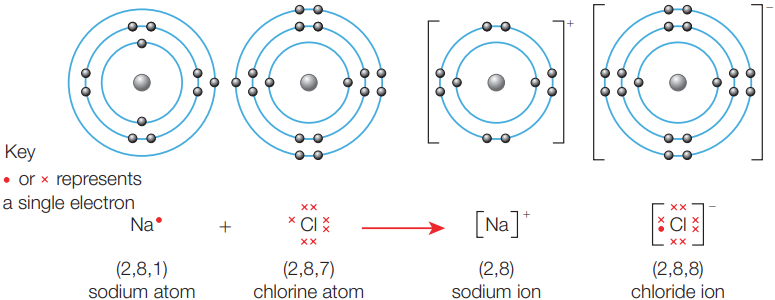
\includegraphics[scale=0.6]{Biology/1A/Images/1A-1-1.png}
        \caption{The formation of sodium chloride.}
    \end{figure}
\end{itemize}

\begin{figure}[H]
    \centering
    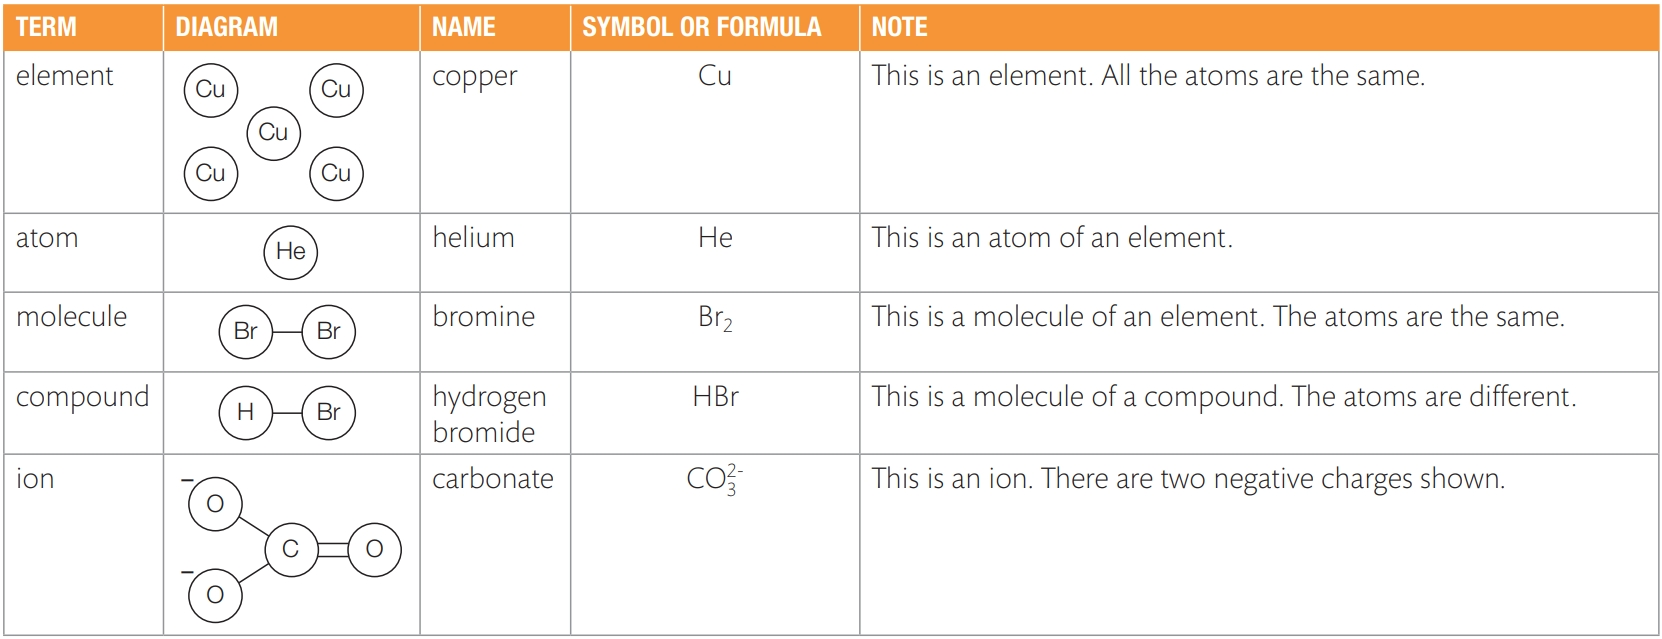
\includegraphics[scale=0.2]{Chemistry/1A/Images/1A-1-1.png}
    \caption{Illustrations of terms used in this chapter.}
\end{figure}

\paragraph{Other Terms}
\begin{itemize}
    \item[1.] \underline{Monatomic} (单原子): Element consisting of single atoms are referred to as monatomic. Example: Helium
    (\ce{He}), a gas used in weather balloons, is a monatomic element.
    \item[2.] \underline{Diatomic} (双原子): Elements and compounds made up of two atoms joined together are called diatomic.
    Common examples include diatomic gases in the atompshere, such as oxygen (\ce{O2}) and nitrogen (\ce{N2}).
    \item[3.] \underline{Polyatomic} (多原子): Elements and compounds made up of molecules containing several atoms joined
    together are described as polyatomic. Examples include sulfuric acid (\ce{H2SO4}) and ammonia (\ce{NH3}).
    \item[4.] Monatomic, Diatomic, and Polyatomic Ions: The same terms apply to ions. Examples include monatomic ion like
    sodium (\ce{Na+}), diatomic ion like hydroixde (\ce{OH-}), and polyatomic ions like sulfate (\ce{SO4^2-}).
\end{itemize}